\subsection{Study datasets}

This study utilized three datasets to demonstrate the common challenges in model evaluation: A null dataset, a simulated spectral dataset, and a real-world spectral dataset. 

\subsubsection{Null dataset}

The null dataset serves as a baseline for the null hypothesis, designed to evaluate the risk of introducing bias in the estimation of model performance. In this dataset, the predictors $X$ and the target variable $y$ are independently drawn from the same normal distribution, ensuring no linear or nonlinear relationship between the input features and the target variable:

\begin{equation} \label{eq_null}
    \begin{cases}
    X \sim \mathcal{N}(0, 1) \\
    y \sim \mathcal{N}(0, 1)
    \end{cases}
\end{equation}

If any model evaluation exercise applied to this dataset produces a significant performance metric, it would indicate a potential bias in the evaluation process. This serves as a critical check to ensure that the evaluation methodology does not artificially inflate the perceived performance of the model.

\subsubsection{Simulated spectral dataset}

To further investigate how these identified challenges impact data with complex structures, both simulated and real spectral datasets were utilized. Spectral data is commonly encountered in agricultural studies, where the target variable is predicted using a series of spectral measurements. This type of data serves as an excellent example for this study because it often presents a significant challenge due to the strong collinearity among predictors. Effectively selecting predictors with reduced correlation is essential to mitigate overfitting and improve model robustness. The simulated spectral dataset was generated following the procedure outlined in \citep{metz_note_2020}, which characterizes spectral signals $X$ as the outcome of a linear combination of a score matrix $T$ and a loading matrix $P$:

\begin{equation} \label{eq_spectral}
    X_{n \times m} = T_{n \times k} P_{m \times k}^\top + E_{n \times m} 
\end{equation}

where $X$ is the spectral data matrix with $n$ samples and $m$ spectral variables, $T$ is the score matrix with $n$ samples and $k$ latent variables, $P$ is the loading matrix with $m$ variables and $k$ latent variables, and $E$ is the residual matrix to simulate noise (Figure ~\ref{fig:1_sim_data}). The $k$ latent variables represent the underlying structure of the spectral data, such as the peaks and valleys in the spectrum. In this study, the spectral data consists of 300 spectral bands ($m = 300$) and four latent variables ($k = 4$). Among these latent variables, only the first two are assumed to contribute meaningfully to the target variable, while the other two are treated as noise.

\begin{figure}[H]
    \centering
    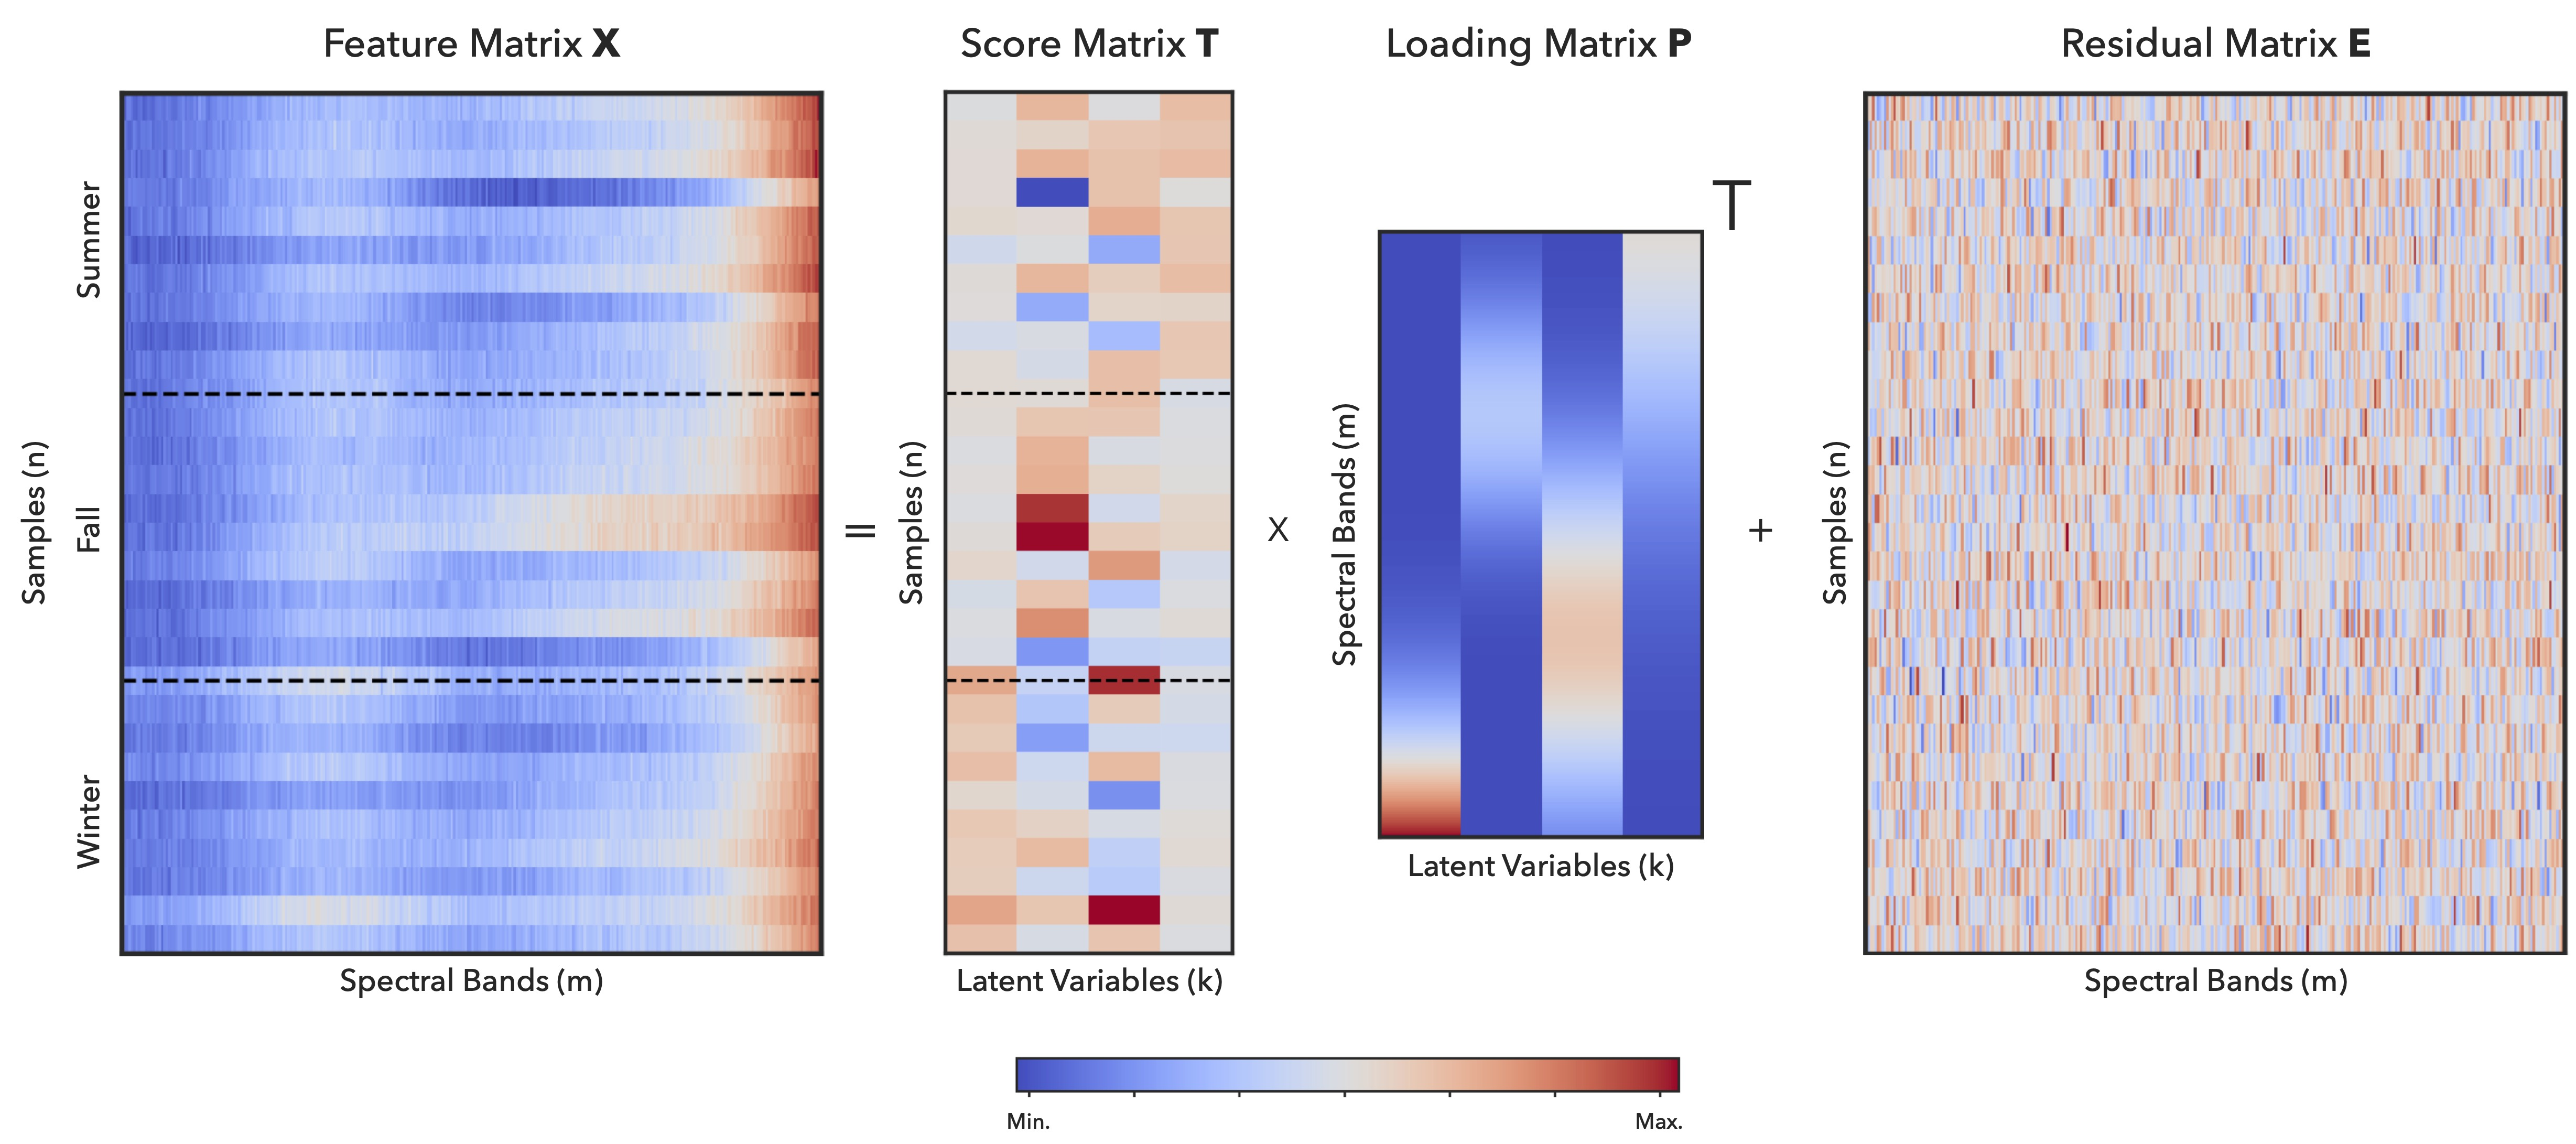
\includegraphics[width=1\textwidth]{fig_1.jpg}
    \caption{Matrix decomposition of the simulated spectral data. The spectral data matrix $X$ is generated as a linear combination of the score matrix $T$ and the loading matrix $P$, with added noise $E$. The color scale is independently normalized for each matrix.}
    \label{fig:1_sim_data}
\end{figure}

The score matrix $T$ defines how each sample contributes to each latent variable. For example, if the third sample exhibits higher spectral measurements around the first peak (as defined by the first latent variable), the value in the third row and first column of the score matrix will be higher relative to other rows. In this study, $T$ was sampled from a multivariate normal distribution with a mean vector of $[1, 1, 1, 1]$ and standard deviations of $[0.02, 0.10, 0.10, 0.02]$. This setup reflects a scenario where the second and third latent variables (corresponding to specific peaks) are more pronounced compared to the first and fourth latent variables. It is inspired by the spectrum measured in the past work \citep{chen_independent_2023}, which used 150 hyperspectral bands ranging from 1,000 nm to 1600 nm to evaluate the wheat kernel quality trait.

The loading matrix $P$ defines how each spectral variable contributes to each latent variable. Each latent variable in $P$ was simulated using a Gaussian probability function with peaks at the -30th, 90th, 200th, and 345th spectral positions and standard deviations of $[100, 40, 60, 60]$ to simulate the width of the peaks. Negative peak positions simulate signals outside the measured spectral range. The residual matrix $E$ is sampled from a normal distribution $\mathcal{N}(0, 0.01)$ to simulate the noise in the spectral data. 

Seasonal variation is an important factor in agricultural studies and is often overlooked in model evaluation. To incorporate this effect, the spectral measurements were simulated across three seasons, with random effects applied to the latent variables. These seasonal effects were modeled by multiplying different scalars with the latent variables in the score matrix $T$. The scalars for the first two latent variables were $[1.00, 1.10, 1.07]$, and for the latter two were $[1.07, 1.00, 1.00]$. This setup reflects a scenario where the first two latent variables are more pronounced in the second and third seasons, while the latter two latent variables dominate in the first season.

The response variable $y$ was generated as a nonlinear function of selected spectral variables. Specifically, four spectral bands ($B$) were selected at indices $[50, 100, 180, 230]$ from the 300 spectral bands. Nonlinear effects were introduced by applying a sinusoidal transformation to the selected spectral variables, raised to the power of three (cubic nonlinearity). To ensure that each effect has a unique sinusoidal component, a phase shift was added to each effect. The phase shift is defined as $\frac{i \pi}{m}$, where $i$ is the index of the selected spectral band, and $m$ is the total number of selected spectral bands. This approach introduces variation in the sinusoidal behavior of each effect, ensuring they are distinct:

$$
y = \sum_{i=1}^{m}\sin(b^3_i + \frac{i \pi}{m}), \quad b_i \in B
$$

where $b_i$ represents the $i$-th selected spectral band from the four bands $B$. Finally, Gaussian noise was added to the response variable $y$ to simulate measurement or modeling errors. The noise was generated with a standard deviation equal to that of the response variable $y$, simulating a scenario where only 50\% of the variance in $y$ can be explained by the spectral data. This approach introduces realistic variability, reflecting the inherent uncertainties and complexities often encountered in real-world prediction tasks.


\begin{figure}[H]
    \centering
    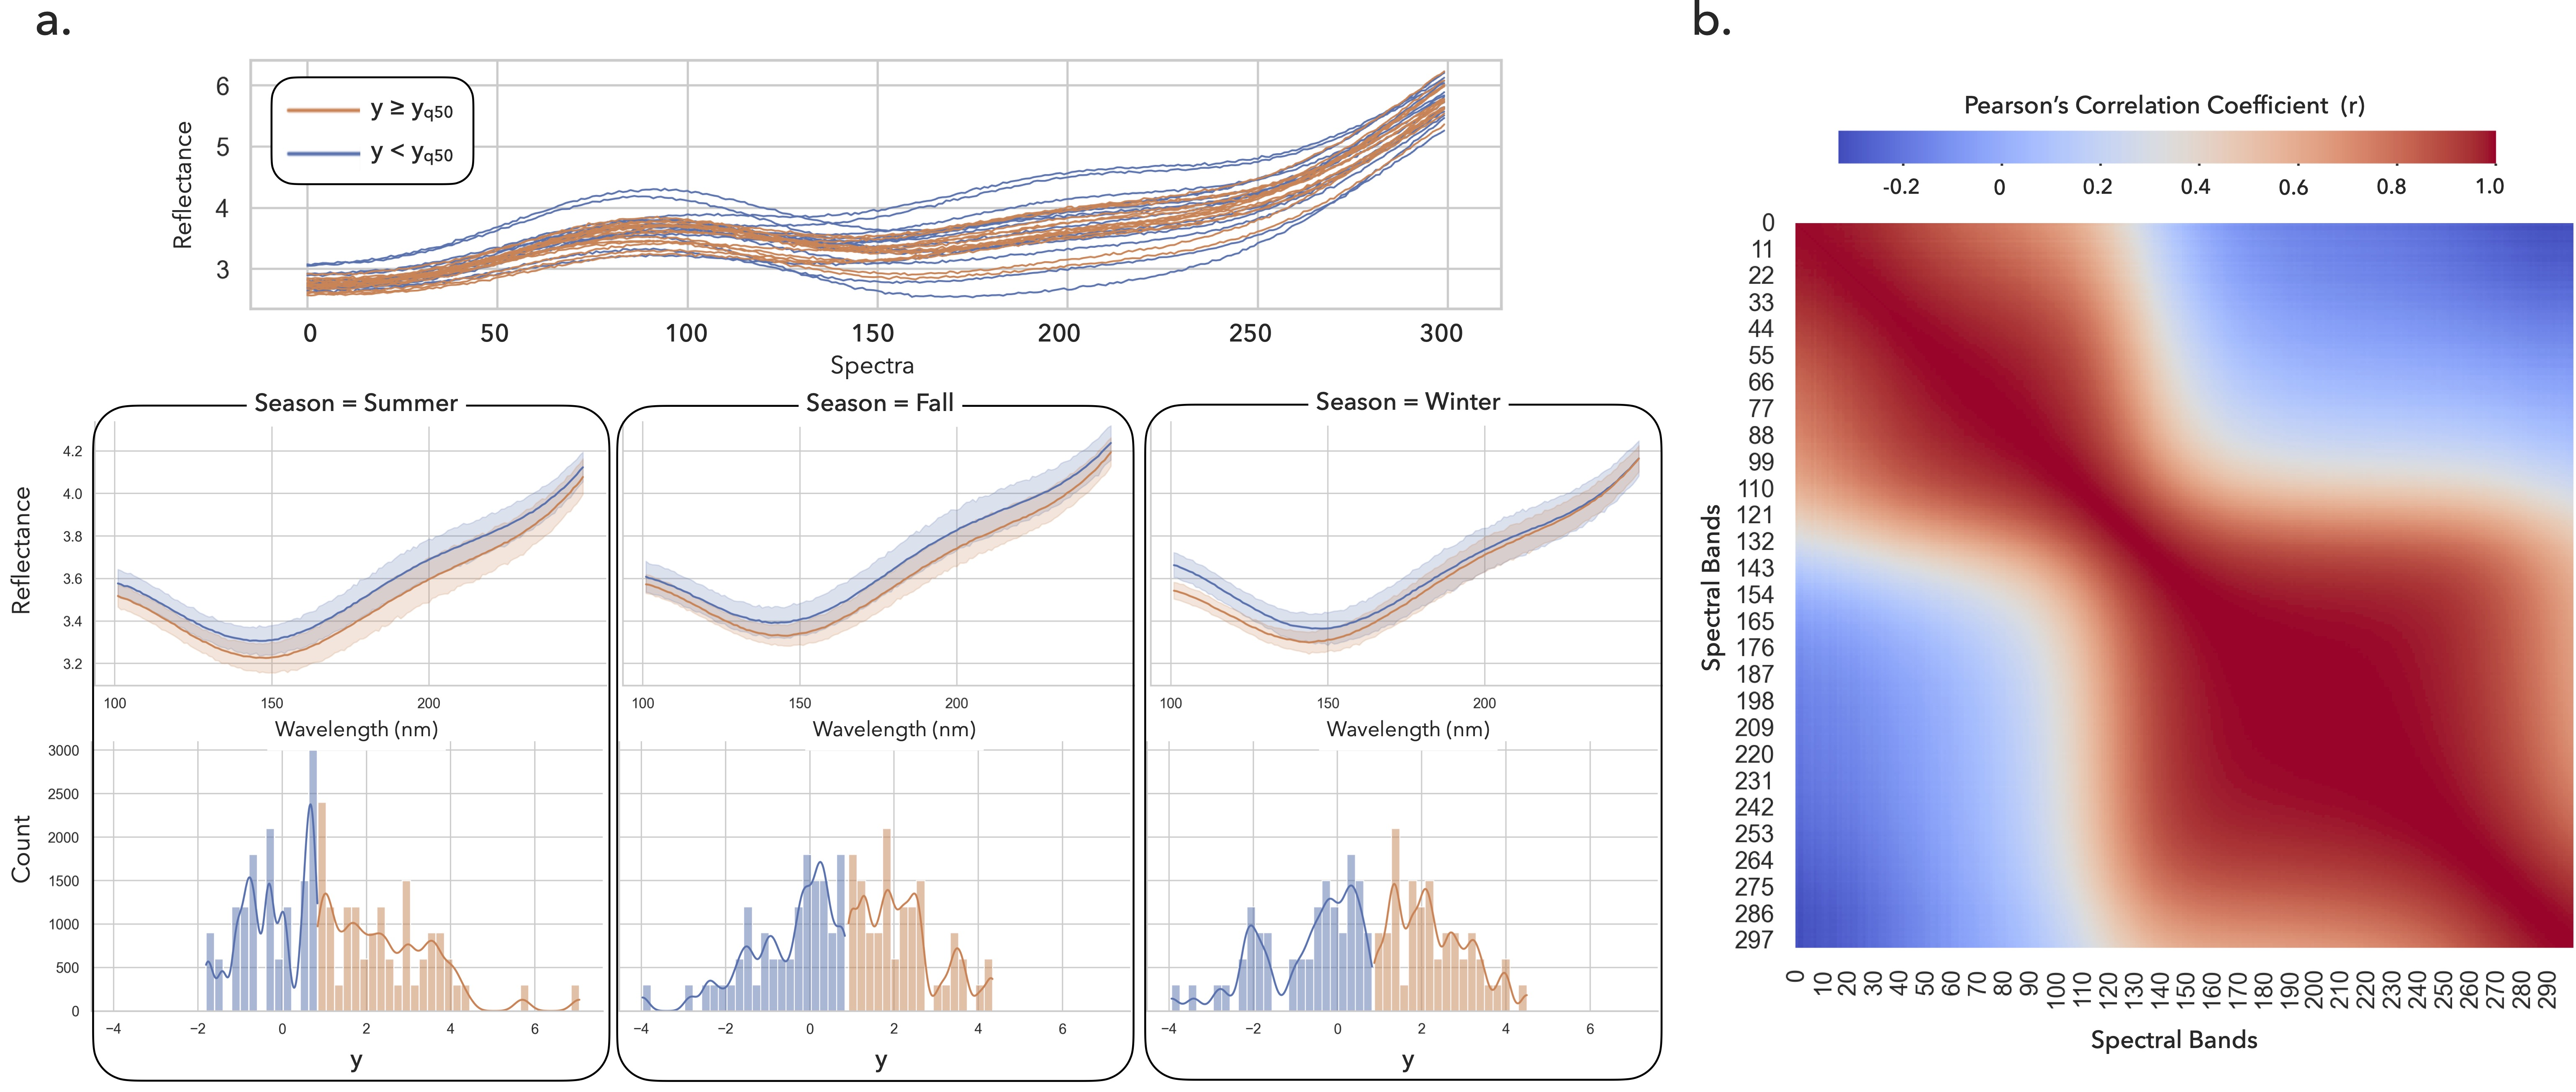
\includegraphics[width=1\textwidth]{fig_2.jpg}
    \caption{Overview of the simulated spectral dataset. (a) The spectral data matrix $X$ is visualized with the target variable $y$ categorized by its median value. (b) The autocorrelation plot of the spectral data matrix $X$ shows a bi-modular structure with the least pair-wise correlation around the 100th band.}
    \label{fig:2_sim_data}
\end{figure}

The simulated spectral data exhibit a bi-modular autocorrelation structure, with the least pair-wise correlation (r=0.4) observed near the 100th band, which serves as the cutoff between the two modules (Figure ~\ref{fig:2_sim_data}b). The non-linear relationship between the spectral data and the target variable $y$ is evident when $y$ is categorized by its median value ($y_{\text{q}50}$) and visualized in two color groups within the spectral space (Figure ~\ref{fig:2_sim_data}a). The resulting plot reveals that the data are not linearly separable in the spectral space, confirming the expected complexity and presenting a challenging task for model evaluation. Additionally, seasonal effects simultaneously influence both the spectral data and the target variable. For instance, the spectral reflection is less pronounced around the 150th band during the first season, while the separability of the two categorical groups decreases around the 250th band in the third season. Furthermore, the distribution of the target variable varies across seasons: the first season displays a right-skewed distribution, whereas the other two seasons have more symmetric distributions. These seasonal variations introduce additional layers of complexity, further highlighting the importance of robust evaluation methods for classification models.

\subsubsection{Real-world spectral dataset}

This dataset contains spectral data collected across 18 bands ranging from 410 nm to 940 nm, aimed at assessing forage quality. The spectral data were captured using a SparkFun ESP32 Thing Plus microprocessor paired with a SparkFun Triad Spectroscopy Sensor (SparkFun Electronics, Niwot, CO). The sensor suite was programmed using Arduino IDE v2.0.4 (Arduino Core Team, 2024) to export measurements.

Forage quality was quantified based on neutral detergent fiber (NDF) content, a critical parameter for evaluating livestock nutrition. Ground truth NDF values were determined using traditional bench chemistry methods with the ANKOM 200 fiber analyzer system (ANKOM Technology, Macedon, NY). The dataset comprises 599 samples collected over three distinct time periods reflecting the seasonal effects on both the spectral data and the NDF response: 189 samples were collected from May to June, 198 from July to August, and 212 from September to October. Sampling took place weekly between May 1 and October 30, 2023, with two samples collected each week from each of 12 fields. Within each field, sampling locations were chosen at random and varied from week to week.

The spectral data were collected in the field using a handheld sensor, while NDF content was measured in the lab. The fields were primarily grazed by cattle, with some fields grazed by other species, including sheep and horses. This dataset provides a comprehensive view of how seasonal variation influences forage quality and spectral characteristics, offering valuable insights into the dynamics of pasture composition and livestock nutrition.

\begin{figure}[H]
    \centering
    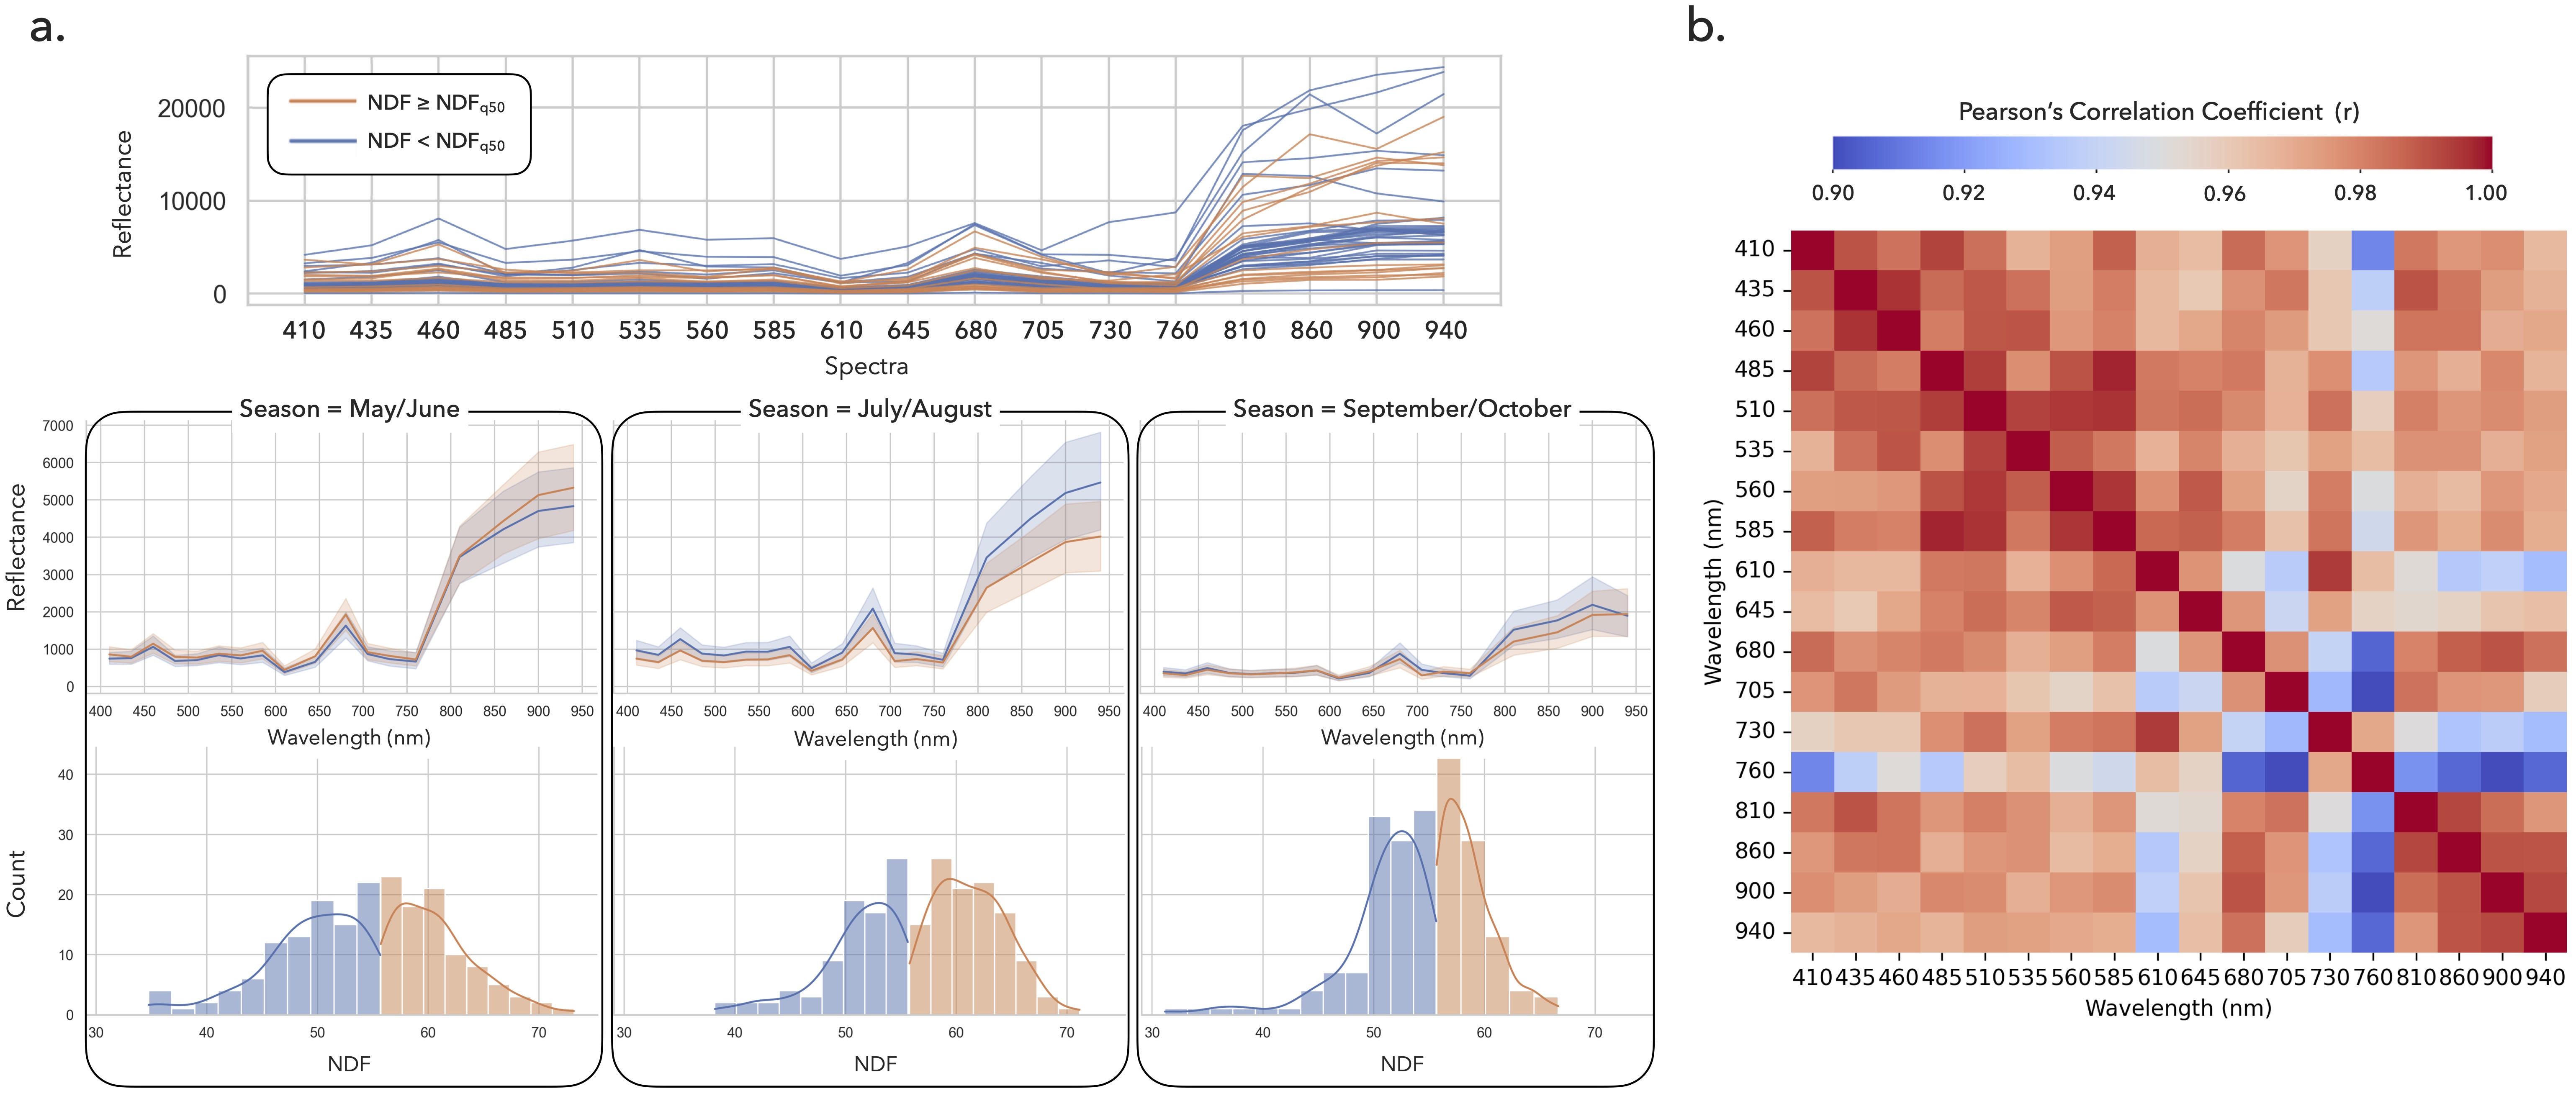
\includegraphics[width=1\textwidth]{fig_3.jpg}
    \caption{Overview of the real spectral dataset. (a) The spectral data matrix $X$ is visualized with the neutral detergent fiber (NDF) $y$ categorized by its median value. (b) The autocorrelation plot of the spectral data matrix $X$.}
    \label{fig:3_real_data}
\end{figure}

A similar examination of the data structure was conducted for both the spectral measurements and the target variable (Figure ~\ref{fig:3_real_data}). The autocorrelation in the spectral measurements is notably stronger than in the simulated dataset, with at least 0.90 for pairwise Pearson correlation coefficients. The seasonal interactions among the spectral measurements are also more pronounced compared to the simulated data. For instance, the spectral reflectance measured in September and October is roughly halved compared to the other seasons. Additionally, a distinct seasonal pattern was observed in the reflectance data beyond 800 nm. In July and August, samples with lower NDF value tend to exhibit higher spectral reflectance, whereas this trend is not evident in May–June or September–October. Moreover, the NDF distribution shows greater variability in July and August, with a higher standard deviation (7.15) compared to May–June (6.19) and September–October (5.23). These observations highlight the stronger seasonal effects and variability in the real dataset compared to the simulated data, providing another example of the challenges in evaluating model performance in real-world agricultural studies.